\chapter{Phương pháp nghiên cứu và thiết kế DepSev-ML}
\label{ch:phuong-phap}

\section{Kiến trúc tổng thể DepSev-ML}
\label{sec:kien-truc-tong-the}

Khung làm việc \textbf{DepSev-ML} (Depression Severity Machine Learning Framework) được thiết kế theo nguyên tắc module hóa, chuẩn tắc hóa và kiểm soát nghiêm ngặt tính toàn vẹn của dữ liệu y tế. Toàn bộ chu trình nghiên cứu từ khâu thu thập dữ liệu thô đến khâu đánh giá mô hình được khái quát hóa thành 7 cấu phần chính trong sơ đồ Hình \ref{fig:overall-architecture}.

\begin{figure}[htbp]{Kiến trúc tổng thể của khung thực nghiệm DepSev-ML}
\centering
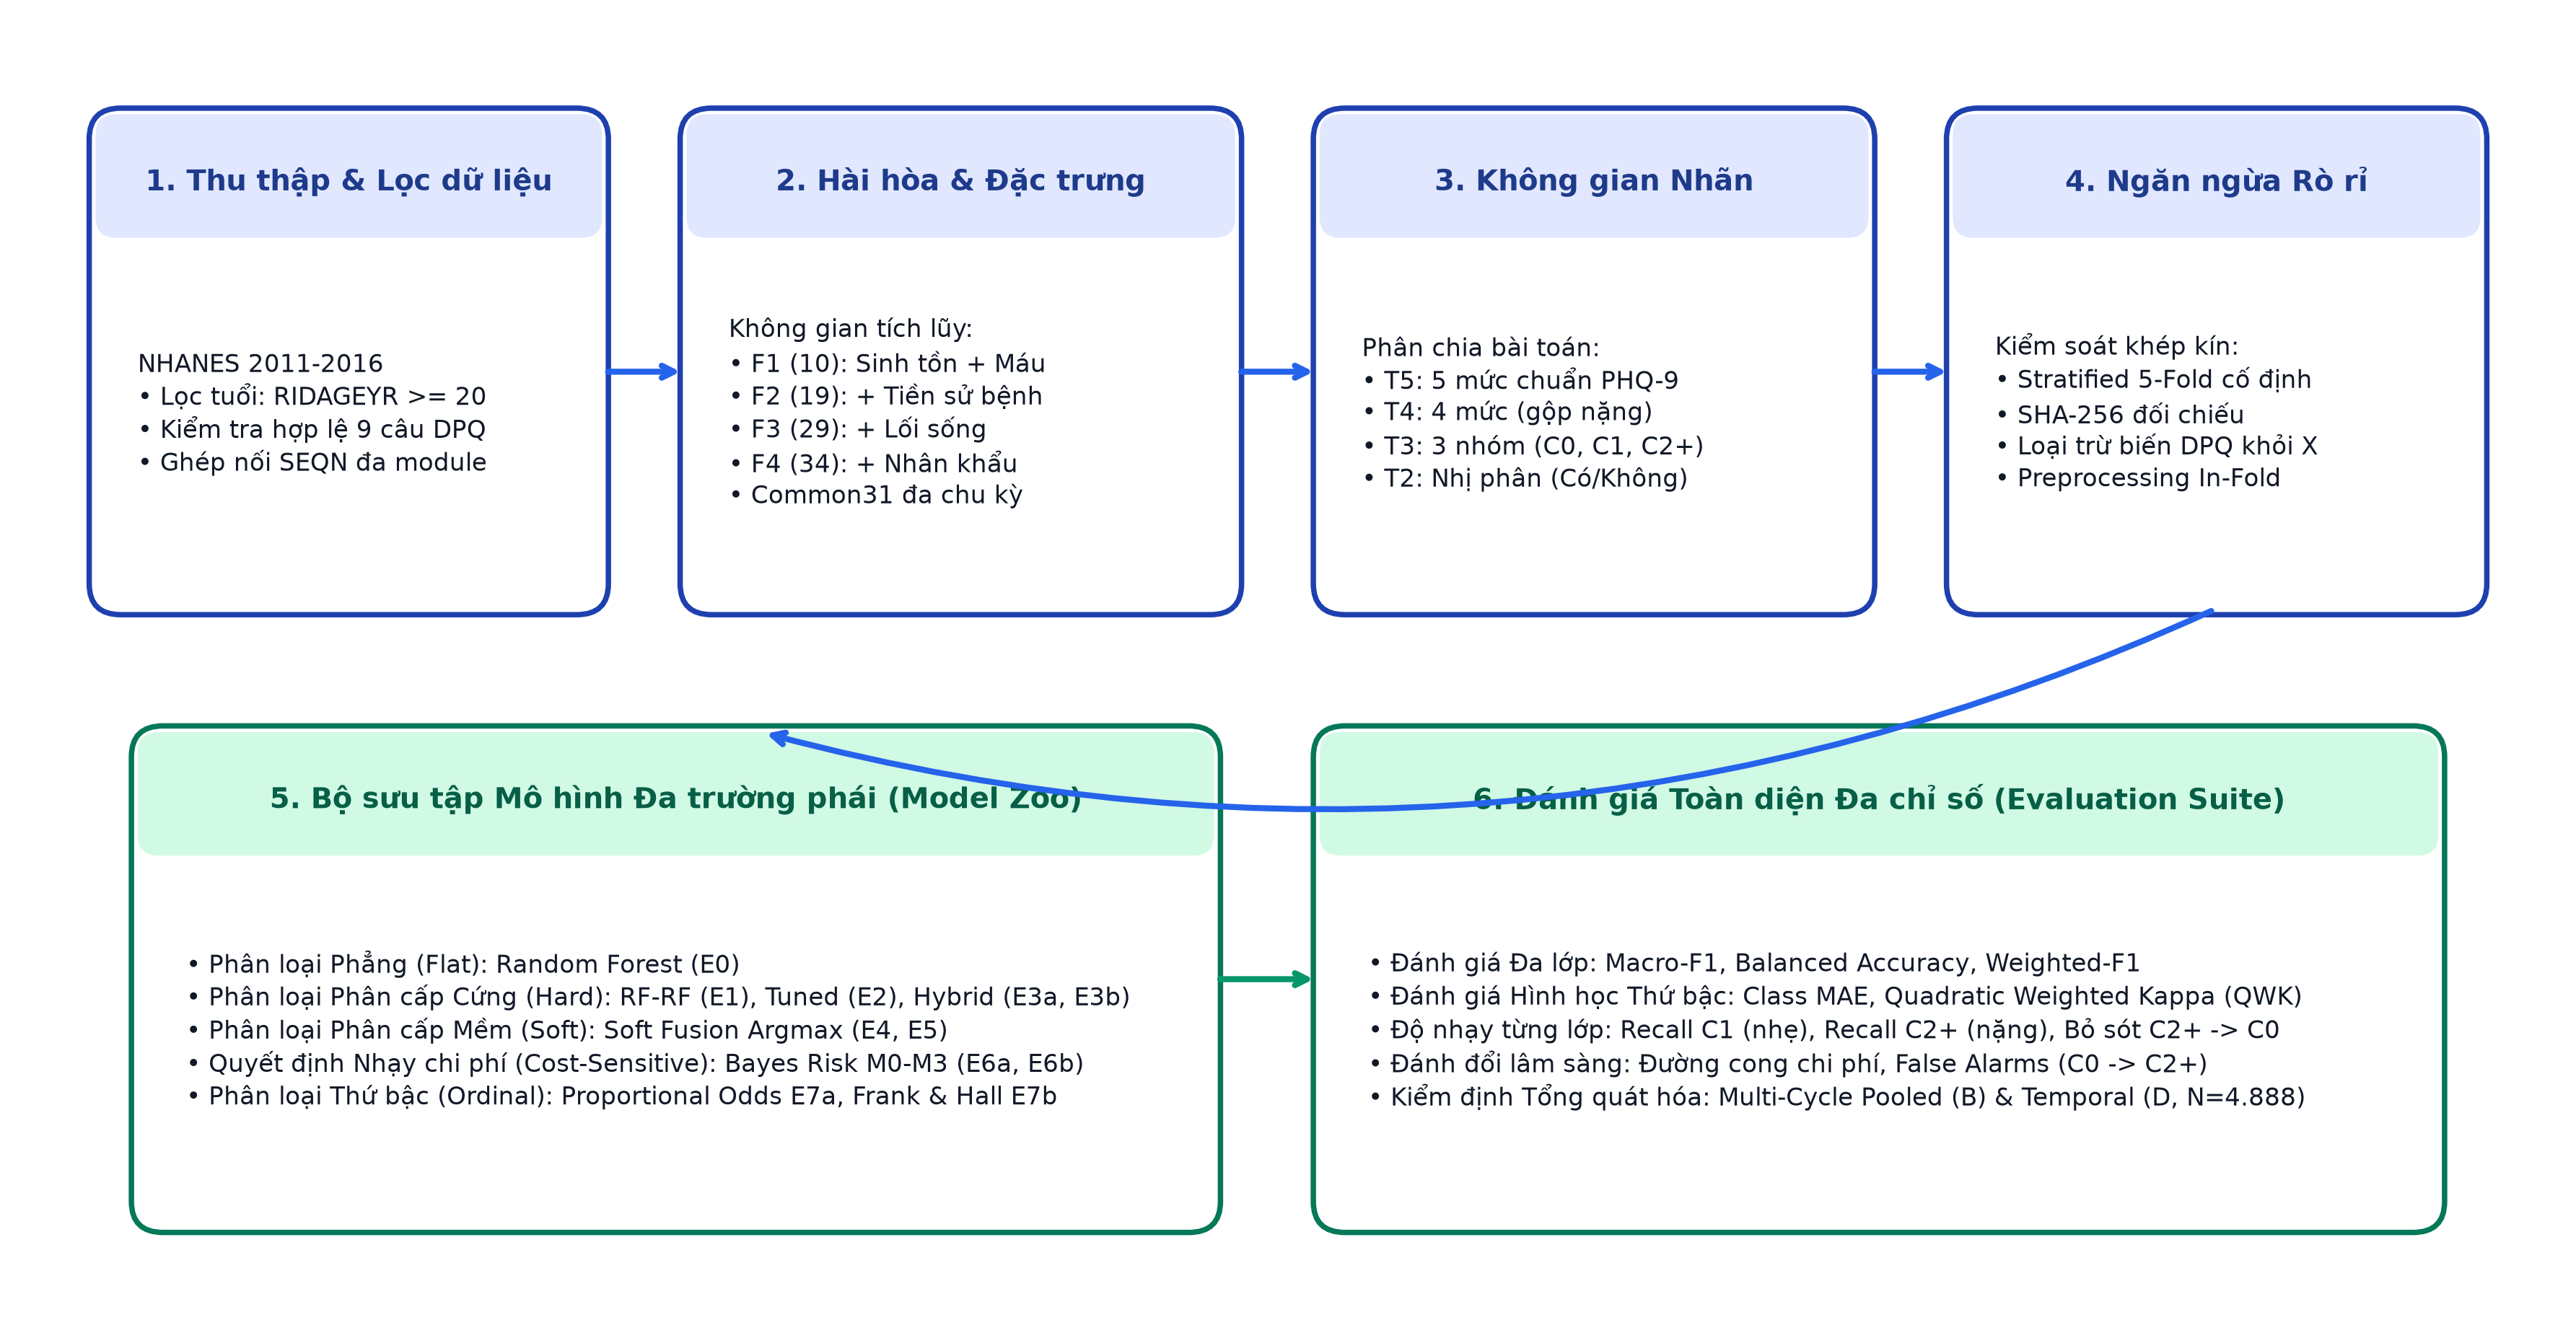
\includegraphics[width=\textwidth]{figures/depsev_overall_architecture.png}
\label{fig:overall-architecture}
\end{figure}
\FloatBarrier

Các cấu phần trong kiến trúc bao gồm:
\begin{enumerate}
    \item \textbf{Data Ingestion \& Filtering:} Tiếp nhận các bảng dữ liệu gốc định dạng SAS Transport (.XPT) hoặc CSV từ NHANES, thực hiện lọc điều kiện người trưởng thành ($\text{RIDAGEYR} \ge 20$) và kiểm tra tính hợp lệ của 9 câu hỏi khảo sát DPQ.
    \item \textbf{Data Harmonization \& Feature Engineering:} Trích xuất các nhóm chỉ số sinh lý, lâm sàng, thói quen sinh hoạt và nhân khẩu học; xử lý chuyển đổi mã hóa các câu hỏi điều hướng phức tạp (như tình trạng hút thuốc và sử dụng rượu bia).
    \item \textbf{Target Construction Module:} Ánh xạ tổng điểm PHQ-9 thành 4 không gian mục tiêu rời rạc ($T_2, T_3, T_4, T_5$).
    \item \textbf{Partitioning \& Isolation Engine:} Quản lý các phân hoạch dữ liệu cố định (Fixed CV Folds, Development/Held-out splits) thông qua mã băm mật mã SHA-256 để bảo đảm khả năng tái lập và ngăn ngừa rò rỉ dữ liệu.
    \item \textbf{Strict In-fold Preprocessing Pipeline:} Thực hiện điền khuyết (median/constant imputation), chuẩn hóa độ lệch chuẩn (StandardScaler) và mã hóa one-hot (OneHotEncoder) nghiêm ngặt bên trong từng training fold.
    \item \textbf{Multi-Paradigm Model Zoo:} Cung cấp các kiến trúc mô hình học máy: Phân loại phẳng (Flat), Phân loại phân cấp (Hard/Soft Hierarchical, Cost-Sensitive Decision) và Phân loại thứ bậc (Ordinal Logistic Regression, Cumulative Binary).
    \item \textbf{Multi-Dimensional Evaluation Suite:} Đánh giá toàn diện trên cả các chỉ số phân loại danh nghĩa (Macro-F1, Balanced Accuracy, Precision/Recall per class) và các chỉ số hình học thứ bậc (Class MAE, Quadratic Weighted Kappa, tỷ lệ lỗi 1 mức và 2 mức).
\end{enumerate}

\section{Dữ liệu nghiên cứu và Hài hòa hóa đa chu kỳ}
\label{sec:du-lieu-nghien-cuu}

Nghiên cứu sử dụng hai tập dữ liệu chính phản ánh hai giai đoạn phát triển của framework:

\subsection{Legacy Development Cohort (NHANES 2013--2014)}
Tập dữ liệu Legacy được xây dựng từ chu kỳ NHANES 2013--2014 kết hợp với tập dữ liệu tiền xử lý chuẩn CDC trên nền tảng Kaggle, có tổng số $N = 5.054$ người tham gia khảo sát đáp ứng điều kiện từ 20 tuổi trở lên và có đầy đủ 9 câu hỏi DPQ:
\begin{itemize}
    \item \textbf{Tập phát triển (Development Partition):} Gồm $N = 4.045$ đối tượng, được sử dụng xuyên suốt cho các thực nghiệm kiểm định chéo Stratified 5-Fold CV, Feature Ablation, Nested CV Tuning, Ensemble và toàn bộ chuỗi thực nghiệm $E_0$--$E_7$.
    \item \textbf{Tập kiểm tra bổ sung (Supplementary Held-out Partition):} Gồm $N = 1.009$ đối tượng được giữ riêng biệt để kiểm tra tham khảo. Cần lưu ý về mặt lai lịch dữ liệu (data provenance): trong quá trình tái cấu trúc phân hoạch chuẩn (split restoration), 813 trong số 1.009 quan sát của tập Held-out từng thuộc tập dữ liệu phát triển ở các phiên bản tiền nghiệm (\texttt{historically\_untouched=false} trong tài liệu kho mã nguồn). Do đó, tập kiểm tra bổ sung này được sử dụng với tính chất đối chứng tham khảo, trong khi toàn bộ các khẳng định hiệu năng khoa học cốt lõi của đề tài được kiểm chứng vững chắc trên quy trình kiểm định chéo Stratified 5-Fold lồng nhau trên tập phát triển ($N = 4.045$).
\end{itemize}

Phân bố nhãn lâm sàng PHQ-9 trên Legacy Cohort được trình bày trong Bảng \ref{tab:legacy-class-dist}.

\begin{table}{Phân bố các lớp triệu chứng PHQ-9 trên Legacy Cohort ($N = 5.054$)}
\centering
\label{tab:legacy-class-dist}
\begin{tabular}{l c c c c c c}
\toprule
\textbf{Phân hoạch} & \textbf{Tổng $N$} & \textbf{$C_0$ (0--4)} & \textbf{$C_1$ (5--9)} & \textbf{$C_2$ (10--14)} & \textbf{$C_3$ (15--19)} & \textbf{$C_4$ (20--27)} \\
\midrule
Development & 4.045 & 3.016 (74.56\%) & 638 (15.77\%) & 243 (6.01\%) & 104 (2.57\%) & 44 (1.09\%) \\
Held-out & 1.009 & 748 (74.13\%) & 162 (16.06\%) & 60 (5.95\%) & 28 (2.78\%) & 11 (1.09\%) \\
\midrule
\textbf{Toàn bộ} & \textbf{5.054} & \textbf{3.764 (74.48\%)} & \textbf{800 (15.83\%)} & \textbf{303 (6.00\%)} & \textbf{132 (2.61\%)} & \textbf{55 (1.09\%)} \\
\bottomrule
\end{tabular}
\end{table}

\subsection{Official Multi-Cycle Cohort (NHANES 2011--2016)}
Để kiểm tra tính tổng quát hóa của các mô hình trên quy mô lớn, nghiên cứu thực hiện quy trình trích xuất và hài hòa hóa dữ liệu (Data Harmonization) từ các bảng dữ liệu gốc chính thức của CDC qua 3 chu kỳ liên tiếp: 2011--2012, 2013--2014 và 2015--2016.

\textbf{Quy trình Hài hòa hóa (Harmonization Protocol):}
Do các chu kỳ NHANES có thể thay đổi thiết kế bảng hỏi hoặc mã định danh biến số phòng xét nghiệm, nghiên cứu đã thực hiện kiểm định schema nghiêm ngặt:
\begin{enumerate}
    \item Ghép nối các bảng module thành phần (Nhân trắc học BMX, Huyết áp BPX, Hóa sinh máu BIOPRO, Huyết học CBC, Cholesterol TCHOL, HDL, HbA1c GHB, Bảng hỏi y tế MCQ, Hút thuốc SMQ, Rượu bia ALQ, Thể lực PAQ, Giấc ngủ SLQ, Nhân khẩu học DEMO và Trầm cảm DPQ) thông qua mã định danh duy nhất SEQN của từng người tham gia.
    \item Loại bỏ các đặc trưng không tương thích: Ví dụ biến số xét nghiệm Triglyceride chỉ được đo trên một phân nhóm mẫu nhịn ăn (fasting sub-sample) ở một số chu kỳ nhất định, gây ra hiện tượng khuyết thiếu cấu trúc (structural missingness) lên tới 50\%; biến này bắt buộc phải loại bỏ để bảo đảm tính nhất quán.
    \item Hợp nhất thành công tập đặc trưng chuẩn $F_{4\_\text{common31}}$ gồm đúng \textbf{31 biến số đồng nhất} trên toàn bộ 3 chu kỳ.
\end{enumerate}

Bảng \ref{tab:multicycle-class-dist} trình bày quy mô và phân bố lớp của các chu kỳ chính thức.

\begin{table}{Phân bố các lớp triệu chứng trên các tập dữ liệu Multi-cycle chính thức}
\centering
\label{tab:multicycle-class-dist}
\begin{tabular}{l c c c c c c}
\toprule
\textbf{Chu kỳ / Phân nhánh} & \textbf{Tổng $N$} & \textbf{$C_0$ (\%)} & \textbf{$C_1$ (\%)} & \textbf{$C_2$ (\%)} & \textbf{$C_3$ (\%)} & \textbf{$C_4$ (\%)} \\
\midrule
NHANES 2011--2012 & 4.639 & 76.12\% & 14.79\% & 5.22\% & 2.61\% & 1.27\% \\
NHANES 2013--2014 (Branch A) & 5.054 & 74.48\% & 15.83\% & 6.00\% & 2.61\% & 1.09\% \\
NHANES 2015--2016 (Branch D Test) & 4.888 & 74.65\% & 17.21\% & 5.03\% & 2.03\% & 1.08\% \\
\midrule
\textbf{Pooled 2011--2016 (Branch B)} & \textbf{14.581} & \textbf{75.06\%} & \textbf{15.96\%} & \textbf{5.42\%} & \textbf{2.41\%} & \textbf{1.15\%} \\
\bottomrule
\end{tabular}
\end{table}

\section{Hệ thống đặc trưng (Feature Spaces)}
\label{sec:he-thong-dac-trung}

Framework DepSev-ML tổ chức 34 biến đầu vào thành 4 nhóm đặc trưng lũy tiến ($F_1 \to F_4$) nhằm phục vụ thực nghiệm cắt bỏ đặc trưng (Feature Ablation Study) theo đúng giao thức chuẩn (\texttt{results/tables/ablation\_feature\_inventory\_final\_protocol.csv}):
\begin{itemize}
    \item \textbf{Nhóm 1 ($F_1$ -- Thể chất, Dấu hiệu sinh tồn \& Xét nghiệm máu, 10 biến):} Gồm 5 chỉ số thể chất và sinh tồn ngoại vi: chỉ số khối cơ thể (BMXBMI), chu vi vòng eo (BMXWAIST), tần số mạch đập khi nghỉ (BPXPLS), trung bình 3 lần đo huyết áp tâm thu (SBP\_mean) và huyết áp tâm trương (DBP\_mean); kết hợp cùng 5 chỉ số xét nghiệm cận lâm sàng máu thiết yếu: Glycohemoglobin HbA1c (LBXGH), Cholesterol toàn phần (LBXTC), HDL-Cholesterol (LBDHDD), Creatinine huyết thanh (LBXSCR) và Albumin huyết thanh (LBXSAL).
    \item \textbf{Nhóm 2 ($F_2$ -- $F_1$ kết hợp Tiền sử bệnh lý lâm sàng, 19 biến):} Bổ sung 9 biến tiền sử bệnh lý và chẩn đoán của bác sĩ: tiền sử tăng huyết áp (BPQ020), đái tháo đường (DIQ010), 5 bệnh lý tim mạch và đột quỵ (MCQ160B, MCQ160C, MCQ160D, MCQ160E, MCQ160F), tiền sử ung thư (MCQ220) và tự đánh giá sức khỏe tổng quát (HUQ010).
    \item \textbf{Nhóm 3 ($F_3$ -- $F_2$ kết hợp Hành vi lối sống \& Giấc ngủ, 29 biến):} Bổ sung 10 chỉ số hành vi sinh hoạt: hoạt động thể lực cường độ mạnh/vừa tại nơi làm việc và giải trí (PAQ605, PAQ620, PAQ650, PAQ665), thời gian ngồi tĩnh tại mỗi ngày (PAD680), tình trạng hút thuốc lá (smoking\_status), thói quen uống rượu bia (ALQ101, alcohol\_status, alcohol\_quantity\_code) và thời lượng giấc ngủ ban đêm (SLD010H).
    \item \textbf{Nhóm 4 ($F_4$ -- Toàn diện kết hợp Nhân khẩu học \& Kinh tế xã hội, 34 biến):} Bổ sung 5 đặc trưng nhân khẩu học quan trọng: Tuổi (RIDAGEYR), Giới tính sinh học (RIAGENDR), Chủng tộc/Dân tộc (RIDRETH1), Trình độ học vấn (DMDEDUC2) và Tỷ lệ thu nhập trên chuẩn nghèo gia đình (INDFMPIR).
\end{itemize}

Trong tập dữ liệu đa chu kỳ $F_{4\_\text{common31}}$, ba biến số không đồng nhất giữa các chu kỳ bị loại bỏ, giữ lại 31 biến số cốt lõi hoàn toàn tương thích. Danh mục chi tiết các biến số được quy định trong Bảng \ref{tab:feature-inventory}.

\begin{longtable}{p{2.5cm} p{2.2cm} p{2.5cm} p{6.5cm}}
\caption{Danh mục hệ thống 34 đặc trưng trong không gian $F_4$ theo giao thức chính thức} \label{tab:feature-inventory} \\
\toprule
\textbf{Mã biến} & \textbf{Nhóm đặc trưng} & \textbf{Kiểu dữ liệu} & \textbf{Mô tả lâm sàng / ý nghĩa} \\
\midrule
\endfirsthead
\toprule
\textbf{Mã biến} & \textbf{Nhóm đặc trưng} & \textbf{Kiểu dữ liệu} & \textbf{Mô tả lâm sàng / ý nghĩa} \\
\midrule
\endhead
\bottomrule
\endfoot
\multicolumn{4}{l}{\textbf{Nhóm $F_1$ (10 đặc trưng): Dấu hiệu sinh tồn, Nhân trắc \& Xét nghiệm máu}} \\
BMXBMI & Thể chất ($F_1$) & Liên tục (kg/m$^2$) & Chỉ số khối cơ thể (Body Mass Index) \\
BMXWAIST & Thể chất ($F_1$) & Liên tục (cm) & Chu vi vòng eo (đo lường béo phì trung tâm) \\
BPXPLS & Sinh tồn ($F_1$) & Rời rạc (nhịp/phút) & Tần số mạch đập khi nghỉ ngơi (60 giây) \\
SBP\_mean & Sinh tồn ($F_1$) & Liên tục (mmHg) & Huyết áp tâm thu trung bình qua các lần đo \\
DBP\_mean & Sinh tồn ($F_1$) & Liên tục (mmHg) & Huyết áp tâm trương trung bình qua các lần đo \\
LBXGH & Cận lâm sàng ($F_1$) & Liên tục (\%) & Glycohemoglobin (HbA1c - chuyển hóa đường) \\
LBXTC & Cận lâm sàng ($F_1$) & Liên tục (mg/dL) & Cholesterol toàn phần huyết thanh \\
LBDHDD & Cận lâm sàng ($F_1$) & Liên tục (mg/dL) & HDL-Cholesterol (cholesterol tỷ trọng cao) \\
LBXSCR & Cận lâm sàng ($F_1$) & Liên tục (mg/dL) & Creatinine huyết thanh (chức năng lọc của thận) \\
LBXSAL & Cận lâm sàng ($F_1$) & Liên tục (g/dL) & Albumin huyết thanh (chức năng gan, dinh dưỡng) \\
\midrule
\multicolumn{4}{l}{\textbf{Nhóm $F_2$ (19 đặc trưng): $F_1$ + 9 tiền sử bệnh lý lâm sàng}} \\
BPQ020 & Tiền sử ($F_2$) & Phân loại nhị phân & Bác sĩ từng chẩn đoán Tăng huyết áp \\
DIQ010 & Tiền sử ($F_2$) & Phân loại nhị phân & Bác sĩ từng chẩn đoán Đái tháo đường \\
MCQ160B & Tiền sử ($F_2$) & Phân loại nhị phân & Bác sĩ từng chẩn đoán Suy tim sung huyết \\
MCQ160C & Tiền sử ($F_2$) & Phân loại nhị phân & Bác sĩ từng chẩn đoán Bệnh tim mạch vành \\
MCQ160D & Tiền sử ($F_2$) & Phân loại nhị phân & Bác sĩ từng chẩn đoán Đau thắt ngực \\
MCQ160E & Tiền sử ($F_2$) & Phân loại nhị phân & Tiền sử từng bị Cơn đau tim / Nhồi máu cơ tim \\
MCQ160F & Tiền sử ($F_2$) & Phân loại nhị phân & Tiền sử từng bị Đột quỵ / Tai biến mạch máu não \\
MCQ220 & Tiền sử ($F_2$) & Phân loại nhị phân & Tiền sử từng được chẩn đoán mắc Ung thư \\
HUQ010 & Lâm sàng ($F_2$) & Thứ bậc (1--5) & Tự đánh giá tình trạng sức khỏe tổng quát \\
\midrule
\multicolumn{4}{l}{\textbf{Nhóm $F_3$ (29 đặc trưng): $F_2$ + 10 hành vi lối sống \& giấc ngủ}} \\
PAQ605, PAQ620 & Lối sống ($F_3$) & Phân loại nhị phân & Hoạt động thể lực cường độ mạnh / vừa tại nơi làm việc \\
PAQ650, PAQ665 & Lối sống ($F_3$) & Phân loại nhị phân & Hoạt động thể lực cường độ mạnh / vừa trong giải trí \\
PAD680 & Lối sống ($F_3$) & Liên tục (phút/ngày) & Thời gian ngồi tĩnh tại trung bình mỗi ngày \\
smoking\_status & Lối sống ($F_3$) & Phân loại 3 mức & Tình trạng hút thuốc lá (Never, Former, Current) \\
ALQ101 & Lối sống ($F_3$) & Phân loại nhị phân & Uống ít nhất 12 đồ uống có cồn trong năm qua \\
alcohol\_status & Lối sống ($F_3$) & Phân loại 3 mức & Tình trạng dùng rượu bia (Non, Moderate, Heavy) \\
alcohol\_qty & Lối sống ($F_3$) & Thứ bậc lượng hóa & Mức độ tiêu thụ rượu bia lượng hóa \\
SLD010H & Lối sống ($F_3$) & Liên tục (giờ) & Thời lượng giấc ngủ thông thường mỗi đêm \\
\midrule
\multicolumn{4}{l}{\textbf{Nhóm $F_4$ (34 đặc trưng): $F_3$ + 5 nhân khẩu học \& kinh tế xã hội}} \\
RIDAGEYR & Nhân khẩu ($F_4$) & Liên tục (tuổi) & Tuổi của người tham gia khảo sát tại thời điểm khám \\
RIAGENDR & Nhân khẩu ($F_4$) & Phân loại nhị phân & Giới tính sinh học (Nam / Nữ) \\
RIDRETH1 & Nhân khẩu ($F_4$) & Phân loại 5 nhóm & Chủng tộc / Dân tộc tự xác định \\
DMDEDUC2 & Nhân khẩu ($F_4$) & Thứ bậc (1--5) & Trình độ học vấn cao nhất đạt được (người lớn) \\
INDFMPIR & Kinh tế ($F_4$) & Liên tục (tỷ số) & Tỷ số thu nhập gia đình trên chuẩn nghèo liên bang \\
\end{longtable}


\section{Tiền xử lý dữ liệu và Quy trình chống rò rỉ (Leakage Controls)}
\label{sec:tien-xu-ly}

Dữ liệu y tế luôn đối mặt với vấn đề giá trị khuyết thiếu (missing data) và sự không đồng nhất về thang đo. Một trong những sai lầm phổ biến nhất trong các nghiên cứu học máy y tế là áp dụng các phép biến đổi dữ liệu (chuẩn hóa, điền khuyết) trên toàn bộ tập dữ liệu trước khi chia fold, dẫn đến việc phân phối của tập kiểm tra bị rò rỉ vào tập huấn luyện (Data Leakage).

Trong DepSev-ML, quy trình tiền xử lý được đóng gói trong một \texttt{scikit-learn Pipeline} hoàn toàn cô lập:
\begin{enumerate}
    \item \textbf{Xử lý biến số liên tục (Numerical Pipeline):}
    \begin{itemize}
        \item Điền khuyết bằng trung vị (Median Imputation): Giá trị trung vị $\tilde{x}_j$ được tính toán \textbf{duy nhất trên tập huấn luyện của fold hiện tại} và được áp dụng để điền các ô trống trên cả tập huấn luyện và tập kiểm tra.
        \item Chuẩn hóa Z-score (Standard Scaling): Biến đổi $z = (x - \mu) / \sigma$ trong đó giá trị trung bình $\mu$ và độ lệch chuẩn $\sigma$ được học hoàn toàn từ tập huấn luyện.
    \end{itemize}
    \item \textbf{Xử lý biến số phân loại (Categorical Pipeline):}
    \begin{itemize}
        \item Điền khuyết bằng hằng số: Các ô khuyết thiếu hoặc không xác định được gán nhãn chuỗi cố định \texttt{"missing\_or\_unknown"}.
        \item Mã hóa One-Hot (OneHotEncoder): Thiết lập tham số \texttt{handle\_unknown='ignore'} và \texttt{sparse\_output=False}. Nếu trên tập kiểm tra xuất hiện một danh mục chưa từng gặp trong tập huấn luyện, vectơ mã hóa one-hot tương ứng sẽ tự động gán toàn bộ bằng 0 mà không gây lỗi thực thi.
    \end{itemize}
    \item \textbf{Loại trừ tuyệt đối các biến mục tiêu DPQ:} Không có bất kỳ câu hỏi nào trong số 9 câu hỏi DPQ hay tổng điểm PHQ-9 được phép xuất hiện trong ma trận đặc trưng $\mathbf{X}$.
\end{enumerate}

Sơ đồ thực thi tiền xử lý bên trong kiểm định chéo được mô tả trong Thuật toán \ref{algo:cv-leakage-free}.

\begin{algorithm}[h!]
\SetAlgoLined
\KwIn{Tập dữ liệu $\mathcal{D} = \{(\mathbf{x}_i, y_i)\}_{i=1}^N$, số lượng folds $K=5$, kiến trúc mô hình $\mathcal{M}$}
\KwOut{Tập hợp dự đoán out-of-fold $\hat{\mathbf{y}}_{\text{oof}}$, các độ đo hiệu năng trung bình}
Khởi tạo phân hoạch Stratified 5-Fold: $\{\mathcal{S}_1, \dots, \mathcal{S}_5\} \leftarrow \text{StratifiedKFold}(\mathcal{D}, K=5, \text{seed}=42)$\;
Khởi tạo mảng dự đoán $\hat{\mathbf{y}}_{\text{oof}} \leftarrow \text{zeros}(N)$\;
\For{$k = 1$ \KwTo $5$}{
    $\mathcal{D}_{\text{val}} \leftarrow \mathcal{S}_k$; \quad $\mathcal{D}_{\text{train}} \leftarrow \mathcal{D} \setminus \mathcal{S}_k$\;
    Khởi tạo Pipeline tiền xử lý $\mathcal{P}_k$\;
    $\mathcal{P}_k.\text{fit}(\mathbf{X}_{\text{train}})$ \tcp*{Chỉ fit trên tập train!}
    $\mathbf{X}_{\text{train\_trans}} \leftarrow \mathcal{P}_k.\text{transform}(\mathbf{X}_{\text{train}})$\;
    $\mathbf{X}_{\text{val\_trans}} \leftarrow \mathcal{P}_k.\text{transform}(\mathbf{X}_{\text{val}})$ \tcp*{Transform tập val bằng tham số của train}
    Huấn luyện mô hình: $\mathcal{M}_k.\text{fit}(\mathbf{X}_{\text{train\_trans}}, \mathbf{y}_{\text{train}})$\;
    Dự đoán trên tập kiểm tra: $\hat{\mathbf{y}}_{\text{val}} \leftarrow \mathcal{M}_k.\text{predict}(\mathbf{X}_{\text{val\_trans}})$\;
    Lưu dự đoán: $\hat{\mathbf{y}}_{\text{oof}}[\mathcal{S}_k] \leftarrow \hat{\mathbf{y}}_{\text{val}}$\;
    Tính toán các chỉ số fold $k$: $\text{Macro-F1}_k, \text{BalAcc}_k, \text{MAE}_k$\;
}
Tính trung bình và độ lệch chuẩn của các chỉ số qua 5 folds\;
\Return{$\hat{\mathbf{y}}_{\text{oof}}$, Bảng tổng hợp hiệu năng}\;
\caption{Quy trình kiểm định chéo Stratified 5-Fold không rò rỉ dữ liệu trong DepSev-ML}
\label{algo:cv-leakage-free}
\end{algorithm}

\subsection{Lưu ý về Thiết kế mẫu khảo sát phức hợp (Complex Survey Design)}
\label{subsec:nhanes-survey-design-note}
Khảo sát NHANES áp dụng thiết kế chọn mẫu xác suất phân tầng, phân cụm nhiều giai đoạn (multistage, stratified, clustered probability sampling) đại diện cho toàn bộ dân số không nằm trong viện của Hoa Kỳ, đi kèm trọng số lấy mẫu (\texttt{WTINT2YR}, \texttt{WTMEC2YR}) và các biến số phân tầng (\texttt{SDMVSTRA}, \texttt{SDMVPSU}). 

Trong khuôn khổ nghiên cứu học máy thực nghiệm tiêu chuẩn của đề tài, các mô hình được tối ưu hóa theo nguyên lý tối thiểu hóa rủi ro thực nghiệm không trọng số (Unweighted Empirical Risk Minimization -- ERM) trên tập mẫu có sẵn, phù hợp với các tiêu chuẩn benchmark học máy y tế hiện hành. Tuy nhiên, về mặt dịch tễ học và suy luận thống kê quần thể chính thống, các ước lượng này không phản ánh hoàn toàn xác suất đại diện dịch tễ trên toàn dân số Hoa Kỳ. Nghiên cứu ghi nhận đây là một giới hạn phương pháp luận quan trọng cần được mở rộng trong tương lai thông qua việc tích hợp hàm hợp lý giả có trọng số (Survey-weighted Pseudo-likelihood).

\section{Thiết kế các mô hình Phân loại phân cấp và Nhạy chi phí}
\label{sec:thiet-ke-hierarchical}

\subsection{Hard Hierarchical Classification ($E_1, E_2, E_3a, E_3b$)}
Hệ thống phân cấp hai tầng cứng hoạt động theo cơ chế tuần tự:
\begin{itemize}
    \item \textbf{Bộ phân loại Tầng 1 ($M_{\text{Stage1}}$):} Được huấn luyện trên toàn bộ tập huấn luyện với nhãn $z_1 = \mathbb{I}(s \ge 5)$. Mục tiêu là phát hiện người có bất kỳ triệu chứng trầm cảm nào.
    \item \textbf{Bộ phân loại Tầng 2 ($M_{\text{Stage2}}$):} Chỉ được huấn luyện trên phân nhóm mẫu có triệu chứng ($s \ge 5$), phân biệt giữa $C_1$ ($s \in [5, 9]$, gán nhãn 0) và $C_2^+$ ($s \in [10, 27]$, gán nhãn 1).
\end{itemize}

Dự đoán được thực hiện theo quy tắc:
\begin{equation}
    \hat{y} = \begin{cases} 0 & \text{nếu } P(Y \ge 1 \mid \mathbf{x}) < \tau_1 \\ 1 & \text{nếu } P(Y \ge 1 \mid \mathbf{x}) \ge \tau_1 \land P(Y = 2 \mid Y \ge 1, \mathbf{x}) < \tau_2 \\ 2 & \text{nếu } P(Y \ge 1 \mid \mathbf{x}) \ge \tau_1 \land P(Y = 2 \mid Y \ge 1, \mathbf{x}) \ge \tau_2 \end{cases}
\end{equation}
Trong mô hình $E_1$, ngưỡng cắt mặc định $\tau_1 = \tau_2 = 0.5$. Trong mô hình $E_2$, hai ngưỡng được tối ưu hóa đồng thời trên không gian lưới thông qua kiểm định chéo nội bộ.

\subsection{Soft Hierarchical kết hợp Tối ưu rủi ro Bayes ($E_4, E_5, E_6a, E_6b$)}
Khắc phục nhược điểm của Hard Routing, mô hình Soft Hierarchical suy diễn phân phối xác suất hợp thành trên toàn bộ không gian 3 lớp thông qua các công thức (\ref{eq:soft-p0})--(\ref{eq:soft-p2}).

Sau khi thu được vectơ xác suất $\mathbf{p}(\mathbf{x}) = [P(C_0), P(C_1), P(C_2^+)]$, quyết định được đưa ra bằng cách tối thiểu hóa rủi ro kỳ vọng theo ma trận chi phí $\mathbf{K}$:
\begin{equation}
    \hat{y} = \arg\min_{j \in \{0, 1, 2\}} \sum_{i=0}^2 P(C_i \mid \mathbf{x}) \cdot K_{ij}
\end{equation}

Bốn ứng viên ma trận chi phí được thiết kế:
\begin{itemize}
    \item \textbf{$M_0$ (Mất mát đồng nhất 0--1, tương đương Argmax):}
    \begin{equation}
        \mathbf{K}_{M0} = \begin{bmatrix} 0 & 1 & 1 \\ 1 & 0 & 1 \\ 1 & 1 & 0 \end{bmatrix}
    \end{equation}
    \item \textbf{$M_1$ (Phạt vừa ca bỏ sót nặng):}
    \begin{equation}
        \mathbf{K}_{M1} = \begin{bmatrix} 0.0 & 1.0 & 1.5 \\ 1.5 & 0.0 & 1.0 \\ 3.0 & 1.5 & 0.0 \end{bmatrix}
    \end{equation}
    \item \textbf{$M_2$ (Phạt nặng ca bỏ sót):}
    \begin{equation}
        \mathbf{K}_{M2} = \begin{bmatrix} 0.0 & 1.0 & 2.0 \\ 2.0 & 0.0 & 1.0 \\ 5.0 & 2.0 & 0.0 \end{bmatrix}
    \end{equation}
    \item \textbf{$M_3$ (Phạt cực đoan ca bỏ sót):}
    \begin{equation}
        \mathbf{K}_{M3} = \begin{bmatrix} 0.0 & 1.0 & 2.5 \\ 2.5 & 0.0 & 1.0 \\ 8.0 & 3.0 & 0.0 \end{bmatrix}
    \end{equation}
\end{itemize}

Thuật toán \ref{algo:soft-cost-sensitive} mô tả chi tiết quy trình dự đoán của mô hình Soft Cost-Sensitive.

\begin{algorithm}[h!]
\SetAlgoLined
\KwIn{Mẫu kiểm tra $\mathbf{x}$, bộ phân loại Tầng 1 $M_{\text{Stage1}}$, bộ phân loại Tầng 2 $M_{\text{Stage2}}$, ma trận chi phí $\mathbf{K}$}
\KwOut{Nhãn dự đoán $\hat{y} \in \{0, 1, 2\}$}
Tính xác suất có triệu chứng: $p_1 \leftarrow M_{\text{Stage1}}.\text{predict\_proba}(\mathbf{x})[:, 1]$\;
Tính xác suất nặng có điều kiện: $p_2 \leftarrow M_{\text{Stage2}}.\text{predict\_proba}(\mathbf{x})[:, 1]$\;
Tích hợp phân phối xác suất 3 lớp:\\
$P(C_0) \leftarrow 1.0 - p_1$\;
$P(C_1) \leftarrow p_1 \cdot (1.0 - p_2)$\;
$P(C_2^+) \leftarrow p_1 \cdot p_2$\;
$\mathbf{P} \leftarrow [P(C_0), P(C_1), P(C_2^+)]$\;
Chuẩn hóa bảo đảm $\sum P(C_k) = 1.0$ và $P(C_k) \ge 0$\;
Tính ma trận rủi ro kỳ vọng: $\mathbf{R} \leftarrow \mathbf{P} \times \mathbf{K}$\;
Chọn nhãn có rủi ro nhỏ nhất: $\hat{y} \leftarrow \arg\min_j R_j$\;
\Return{$\hat{y}$}\;
\caption{Quy trình suy diễn xác suất mềm và quyết định nhạy chi phí ($E_6$)}
\label{algo:soft-cost-sensitive}
\end{algorithm}

\section{Thiết kế các mô hình Phân loại thứ bậc ($E_7$)}
\label{sec:thiet-ke-ordinal}

\subsection{E7a – Ordinal Logistic Regression (Proportional Odds)}
Để bảo đảm tính ổn định và tính tự chủ công nghệ tuyệt đối trên Python 3.13, mô hình \texttt{OrdinalLogisticRegression} được hiện thực trực tiếp từ nguyên lý biến tiềm ẩn. 

\textbf{Tái tham số hóa khử ràng buộc bảo đảm tính đơn điệu:}
Hai ngưỡng cắt $\theta_0$ và $\theta_1$ bắt buộc phải thỏa mãn $\theta_0 < \theta_1$. Thay vì giải bài toán tối ưu có ràng buộc phức tạp, nghiên cứu áp dụng kỹ thuật đổi biến số mũ:
\begin{align}
    \theta_0 &= \alpha \\
    \theta_1 &= \alpha + \exp(\delta), \quad \text{với } \alpha \in \mathbb{R}, \delta \in \mathbb{R}
\end{align}
Khi đó, hiệu số $\theta_1 - \theta_0 = \exp(\delta) > 0$ được bảo đảm luôn dương nghiêm ngặt với mọi giá trị của $\delta \in (-\infty, +\infty)$. Không gian tối ưu trở thành không gian tự do $\mathbb{R}^{d+2}$ đối với vectơ tham số $\mathbf{\Theta} = [\mathbf{w}^T, \alpha, \delta]^T$.

\textbf{Hàm mất mát và Gradient giải tích:}
Hàm mất mát Negative Log-Likelihood có trọng số mẫu $s_i$ và điều chuẩn $L_2$ trên vectơ trọng số $\mathbf{w}$ (không phạt các ngưỡng cắt):
\begin{equation}
    \mathcal{L}(\mathbf{w}, \alpha, \delta) = - \sum_{i=1}^N s_i \log P(Y = y_i \mid \mathbf{x}_i) + \frac{1}{2C} \|\mathbf{w}\|^2
\end{equation}

Đặt $z_{0i} = \alpha - \mathbf{w}^T \mathbf{x}_i$ và $z_{1i} = \alpha + e^\delta - \mathbf{w}^T \mathbf{x}_i$. Xác suất tương ứng là $\sigma_{0i} = \sigma(z_{0i})$ và $\sigma_{1i} = \sigma(z_{1i})$. Đạo hàm riêng giải tích theo từng tham số được dẫn xuất chính xác:
\begin{align}
    \frac{\partial \mathcal{L}}{\partial \mathbf{w}} &= - \sum_{i=1}^N s_i (g_{0i} + g_{1i}) \mathbf{x}_i + \frac{1}{C} \mathbf{w} \\
    \frac{\partial \mathcal{L}}{\partial \alpha} &= \sum_{i=1}^N s_i (g_{0i} + g_{1i}) \\
    \frac{\partial \mathcal{L}}{\partial \delta} &= e^\delta \sum_{i=1}^N s_i g_{1i}
\end{align}
trong đó các đại lượng $g_{0i}, g_{1i}$ được tính theo nhãn thực tế $y_i$:
\begin{equation}
    (g_{0i}, g_{1i}) = \begin{cases} (-(1 - \sigma_{0i}), 0) & \text{nếu } y_i = 0 \\ \left(\frac{\sigma_{0i}(1 - \sigma_{0i})}{\sigma_{1i} - \sigma_{0i}}, -\frac{\sigma_{1i}(1 - \sigma_{1i})}{\sigma_{1i} - \sigma_{0i}}\right) & \text{nếu } y_i = 1 \\ (0, \sigma_{1i}) & \text{nếu } y_i = 2 \end{cases}
\end{equation}

Mô hình được tối ưu hóa bằng thuật toán L-BFGS-B với độ chính xác cao.

\subsection{E7b – Cumulative Binary Classification (Frank \& Hall 2001)}
Quy trình huấn luyện và suy diễn của phương pháp Frank \& Hall kết hợp phép chiếu bình phương tối thiểu được mô tả trong Thuật toán \ref{algo:frank-hall}.

\begin{algorithm}[h!]
\SetAlgoLined
\KwIn{Mẫu kiểm tra $\mathbf{x}$, bộ phân loại $M_1$ dự đoán $P(Y \ge 1)$, bộ phân loại $M_2$ dự đoán $P(Y \ge 2)$}
\KwOut{Phân phối xác suất hợp lệ $\mathbf{p} = [P(C_0), P(C_1), P(C_2^+)]$}
Dự đoán xác suất thô: $q_1 \leftarrow M_1.\text{predict\_proba}(\mathbf{x})[:, 1]$; \quad $q_2 \leftarrow M_2.\text{predict\_proba}(\mathbf{x})[:, 1]$\;
\eIf{$q_2 > q_1$ \tcp*{Vi phạm tính đơn điệu!}}{
    Ghi nhận vi phạm đơn điệu (Monotonicity Violation)\;
    Áp dụng phép chiếu bình phương tối thiểu đẳng điệu:\\
    $q_1' \leftarrow \frac{q_1 + q_2}{2}$; \quad $q_2' \leftarrow \frac{q_1 + q_2}{2}$\;
}{
    $q_1' \leftarrow q_1$; \quad $q_2' \leftarrow q_2$\;
}
Tính xác suất từng lớp:\\
$P(C_0) \leftarrow 1.0 - q_1'$\;
$P(C_1) \leftarrow q_1' - q_2'$\;
$P(C_2^+) \leftarrow q_2'$\;
\Return{$[P(C_0), P(C_1), P(C_2^+)]$}\;
\caption{Quy trình suy diễn Frank \& Hall với phép chiếu đẳng điệu ($E_7b$)}
\label{algo:frank-hall}
\end{algorithm}

\section{Hệ thống thước đo đánh giá (Evaluation Metrics)}
\label{sec:he-thong-thuoc-do}

Để đánh giá toàn diện và phản ánh đúng bản chất bài toán mất cân bằng lớp và phân loại có thứ tự, DepSev-ML sử dụng hệ thống độ đo đa chiều:

\subsection{Các chỉ số phân loại danh nghĩa}
\begin{enumerate}
    \item \textbf{Độ chính xác (Accuracy):}
    \begin{equation}
        \text{Accuracy} = \frac{1}{N} \sum_{i=1}^N \mathbb{I}(y_i = \hat{y}_i)
    \end{equation}
    \textit{Lưu ý phương pháp luận:} Trên dữ liệu mất cân bằng ($C_0$ chiếm 75\%), một mô hình tầm thường (trivial majority baseline) dự đoán toàn bộ là $C_0$ vẫn đạt Accuracy = 74.56\%, nhưng hoàn toàn vô giá trị về mặt y tế. Do đó Accuracy không thể được sử dụng làm chỉ số quyết định.
    \item \textbf{Độ chính xác cân bằng (Balanced Accuracy):}
    \begin{equation}
        \text{Balanced Accuracy} = \frac{1}{K} \sum_{k=0}^{K-1} \text{Recall}_k = \frac{1}{K} \sum_{k=0}^{K-1} \frac{\text{TP}_k}{\text{TP}_k + \text{FN}_k}
    \end{equation}
    Độ đo này triệt tiêu hoàn toàn ưu thế kích thước của lớp đa số bằng cách tính trung bình cộng không trọng số của độ nhạy (Recall) trên từng lớp riêng biệt. Đối với mô hình tầm thường dồn lớp, Balanced Accuracy chỉ đạt đúng $1/K$ (33.33\% trên $T_3$ hoặc 20.0\% trên $T_5$).
    \item \textbf{Macro-averaged F1-score (Macro-F1):}
    \begin{equation}
        \text{Macro-F1} = \frac{1}{K} \sum_{k=0}^{K-1} \text{F1}_k = \frac{1}{K} \sum_{k=0}^{K-1} \frac{2 \cdot \text{Precision}_k \cdot \text{Recall}_k}{\text{Precision}_k + \text{Recall}_k}
    \end{equation}
    Đóng vai trò là \textbf{thước đo chất lượng chính (Primary Metric)} của toàn bộ nghiên cứu.
\end{enumerate}

\subsection{Các chỉ số khoảng cách thứ bậc (Ordinal Metrics)}
\begin{enumerate}
    \item \textbf{Sai số tuyệt đối trung bình theo lớp (Class MAE):}
    \begin{equation}
        \text{Class MAE} = \frac{1}{N} \sum_{i=1}^N |y_i - \hat{y}_i|
    \end{equation}
    với $y_i, \hat{y}_i \in \{0, 1, \dots, K-1\}$. Cần phân biệt rõ: Class MAE được tính trên không gian chỉ số lớp nguyên rời rạc, \textbf{không phải sai số MAE trên tổng điểm PHQ-9 liên tục} $s \in [0, 27]$.
    \item \textbf{Hệ số Kappa Cohen trọng số bậc hai (Quadratic Weighted Kappa -- QWK) \cite{cohen1968weighted}:}
    \begin{equation}
        \kappa_w = 1 - \frac{\sum_{i,j} W_{ij} O_{ij}}{\sum_{i,j} W_{ij} E_{ij}}
    \end{equation}
    trong đó $O_{ij}$ là ma trận nhầm lẫn quan sát được, $E_{ij}$ là ma trận kỳ vọng ngẫu nhiên, và ma trận trọng số phạt bậc hai $W_{ij} = \frac{(i - j)^2}{(K - 1)^2}$. QWK phạt các sai lầm cách xa nhau theo bình phương khoảng cách thứ bậc.
    \item \textbf{Tỷ lệ lỗi 1 mức và lỗi 2 mức (1-Step and 2-Step Error Rates):}
    \begin{align}
        \text{Error}_{\text{1-step}} &= \frac{1}{N} \sum_{i=1}^N \mathbb{I}(|y_i - \hat{y}_i| = 1) \\
        \text{Error}_{\text{2-step}} &= \frac{1}{N} \sum_{i=1}^N \mathbb{I}(|y_i - \hat{y}_i| = 2)
    \end{align}
    Trong đó, các ca sai lệch 2 mức bao gồm hai hướng đối lập: $C_2^+ \to C_0$ (Bỏ sót bệnh nhân nặng sang bình thường) và $C_0 \to C_2^+$ (Báo động giả người bình thường thành rất nặng).
\end{enumerate}

\section{Tóm tắt chương và kết nối thực nghiệm}
\label{sec:tom-tat-chuong-3}

Chương \ref{ch:phuong-phap} đã hoàn thiện việc đặc tả toàn bộ phương pháp luận và thiết kế thực nghiệm của khung làm việc DepSev-ML. Nghiên cứu đã thiết lập một chu trình xử lý dữ liệu chuẩn hóa từ hai tập dữ liệu độc lập: Legacy Cohort ($N=5.054$) phục vụ huấn luyện và kiểm định chéo Stratified 5-Fold không rò rỉ, và Harmonized Multi-Cycle Cohort ($N=14.581$) phục vụ đánh giá quy mô lớn và kiểm tra suy giảm hiệu năng theo thời gian (Temporal Evaluation). Hệ thống 31 đặc trưng chung được cấu trúc lũy tiến thành các tập $F_1 \to F_4$, kết hợp cùng quy trình chuẩn hóa và điền khuyết nghiêm ngặt in-fold. Đồng thời, nghiên cứu đã xây dựng một sở thú mô hình đa trường phái bao gồm Flat Classification, Hard Hierarchical ($E_1$--$E_3$), Soft Hierarchical ($E_4$--$E_5$), Cost-Sensitive Decision ($E_6$), và Ordinal Classification ($E_7$), đi kèm hệ thống chỉ số đánh giá đa chiều (Macro-F1, Balanced Accuracy, Class MAE, QWK, và lỗi sai lệch 1--2 mức).

Toàn bộ các quy tắc thực nghiệm, phân hoạch tập dữ liệu và mô hình được đặc tả trong chương này là cơ sở duy nhất để triển khai các phân tích thực nghiệm và đối chiếu số liệu trong Chương \ref{ch:ket-qua-thao-luan}.
\cleardoublepage
